In this chapter, we analyze the results from the second experiments group: the participant selection techniques. In here, we compare random participant selection with a "first come, first served" basis, where the clients take initiative to join the round.

\section{Client Participation}

In both techniques, there is a factor of randomness. In random selection, both the amount of clients, as well as the clients themselves, are chosen randomly. In "first come, first served", only the amount of clients $C$ is chosen randomly. Then, after $C$ clients submit their updates, the round moves onto the next phase. This difference leads to the question: is the distribution of client participation going to be different? If so, how does it impact the model?

\begin{figure}[!ht]
    \centering
    \centering
    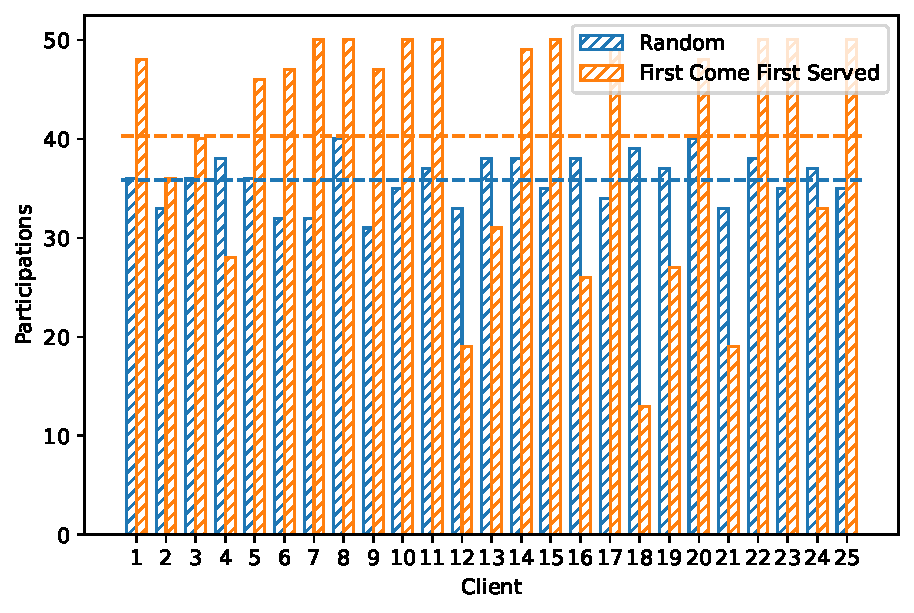
\includegraphics[width=0.7\textwidth]{graphics/selection/clients.pdf}
    \caption{Participation of Each Client Per Selection Technique}
    \label{fig:participations_client}
\end{figure}

To answer the questions, we first need to collect how many times each client participated in a round. On \autoref{fig:participations_client}, we can visualize how many times each client participated, represented by the bars, as well as the average amount of participation per client, represented by the lines. It is clear from the plot that the distributions are different. While the random selection presents a more uniform distribution, where each client was selected a similar amount of times, the "first come first served" selection presents more opposites, where some clients participate a high amount of times and others few times. The values of the standard deviation support this conclusion: for random selection, the standard deviation is approximately 2.49, while for "first come first served" it is 11.84.

This leads us to conclude that, by letting clients taking initiative to join a round, it is possible that some will end up participating more than others. In a system with heterogeneous devices, where some have more computation power than others, this may reveal to be an issue. Since more powerful devices are able to finish the training process faster, they are able to join the round earlier, allowing them to participate more times. By participating more times, they will have more influence over the global model in the end. This is not always desired as it may lead to skewed results.

\section{Execution Time, Transaction Cost and Latency}

Regarding execution time, we can see on \autoref{tab:metrics_selection} that both techniques only differ in around $1.2$ minutes, which translates to a difference of around $1.1$ seconds per round. We can see that random participation is faster than "first come first served". This small difference is likely caused by the fact that, in random selection, less participants participated on average per round, as seen in the previous section. With slightly less participants, it is expected for a round to take slightly less time.

\begin{table}[!ht]
\begin{tabular}{c|c|c} \hline \hline
                              & First Come First Served & Random \\ \hline \hline
E2E Time (m)                   & 19.70                   & 18.93  \\ \hline
Mean Round Time (s)            & 23.62                   & 22.70  \\ \hline
% Median Round Time (s)          & 22.06                   & 21.90  \\ \hline
Mean Transaction Latency (s)   & 1.560                   & 1.549  \\ \hline
% Median Transaction Latency (s) & 1.561                   & 1.549  \\ \hline
Mean Transaction Cost (Gas)    & 189179                  & 183124 \\ \hline
% Median Transaction Cost (Gas)  & 223471                  & 185198 \\ \hline
\end{tabular}
\caption{Time and Transaction Metrics Per Participant Selection Technique}
\label{tab:metrics_selection}
\end{table}

\section{Accuracy and Convergence}

When it comes to accuracy and convergence, we can see the data presented on \autoref{fig:accuracy_selection}. Even though both techniques reached virtually identical accuracy values in the end, random selection was more stable during the initial 20 rounds. This can be explained by the fact that the distribution of devices participating in each round with random selection was more uniform. Since the data is \textit{non-iid}, by having the same clients participate over and over, the model can become skewed. However, after 20 rounds, the majority of the devices had the opportunity to participate in the model, which explains why it became more and more stable.

\begin{figure}[!ht]
    \centering
    \centering
    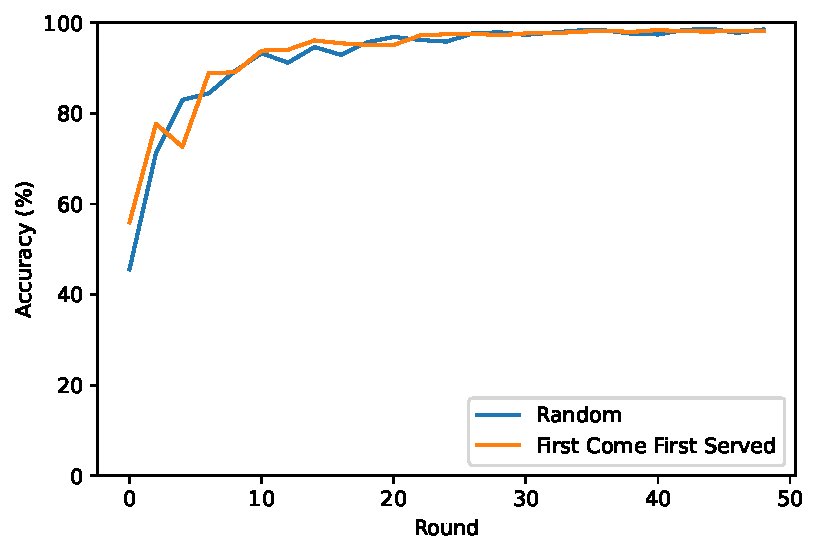
\includegraphics[width=0.7\textwidth]{graphics/selection/accuracy.pdf}
    \caption{Accuracy Per Participant Selection Technique}
    \label{fig:accuracy_selection}
\end{figure}

\section{Communication and Computation Costs}

Regarding communication and computation costs, it is expected that both techniques have similar results. On \autoref{fig:net_selection}, \autoref{fig:ram_selection} and \autoref{fig:cpu_selection}, we can visualize the network traffic per round, RAM usage and CPU usage, respectively, per each of the different devices. This techniques solely influences which and how many participants are selected per round. Therefore, the individual communication traffic is not expected to change significantly as long as the number of participants per round does not change significantly, which can be seen in the figures. In \Cref{chapter:analysis:participants}, we analyze in detail how much different amounts of participants actually impact communication and computation costs.

\begin{figure}[!ht]
    \centering
    \centering
    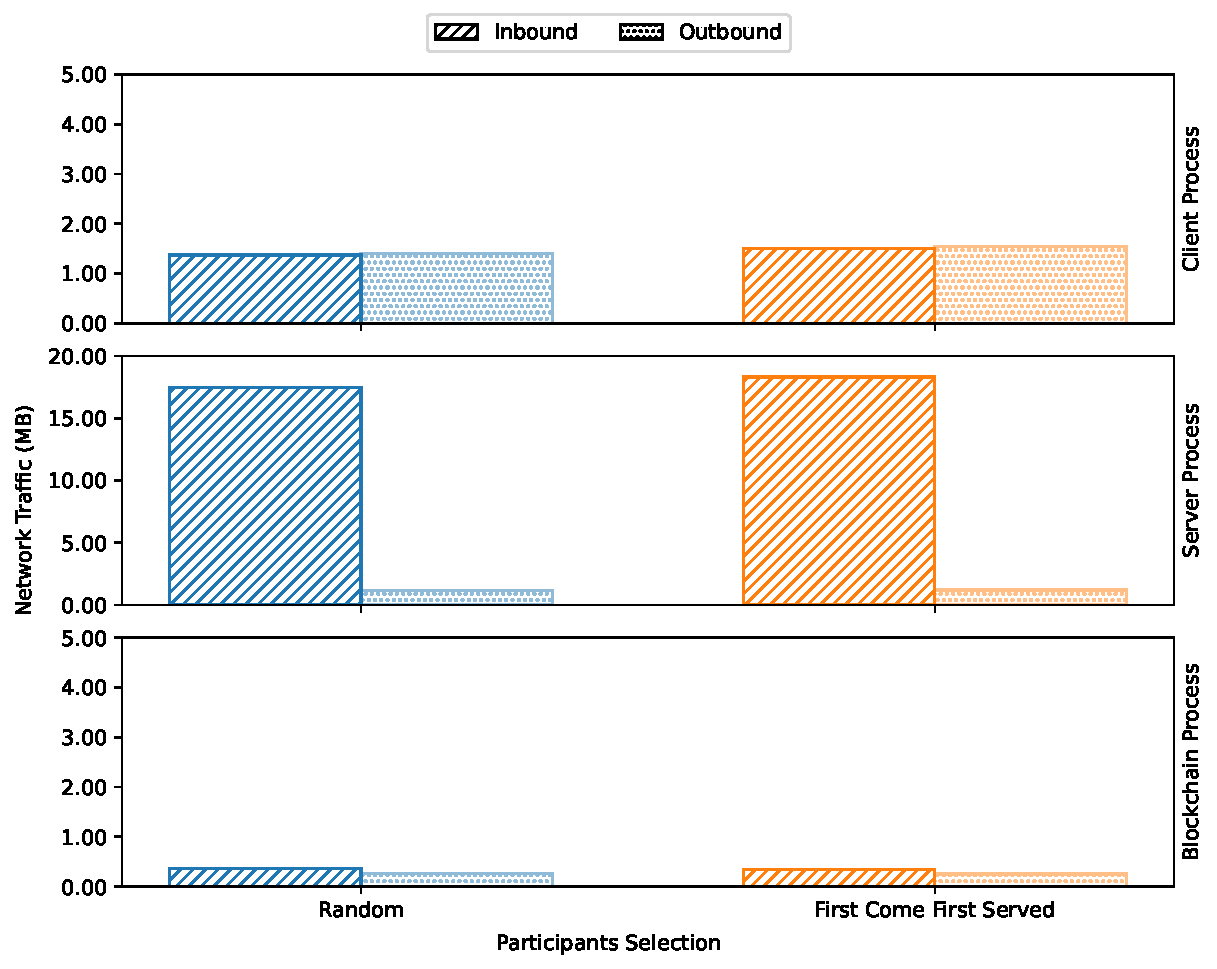
\includegraphics[width=0.8\textwidth]{graphics/selection/net.pdf}
    \caption{Network Traffic Per Round Per Participant Selection Technique}
    \label{fig:net_selection}
\end{figure}

\begin{figure}[!hpt]
    \centering
    \centering
    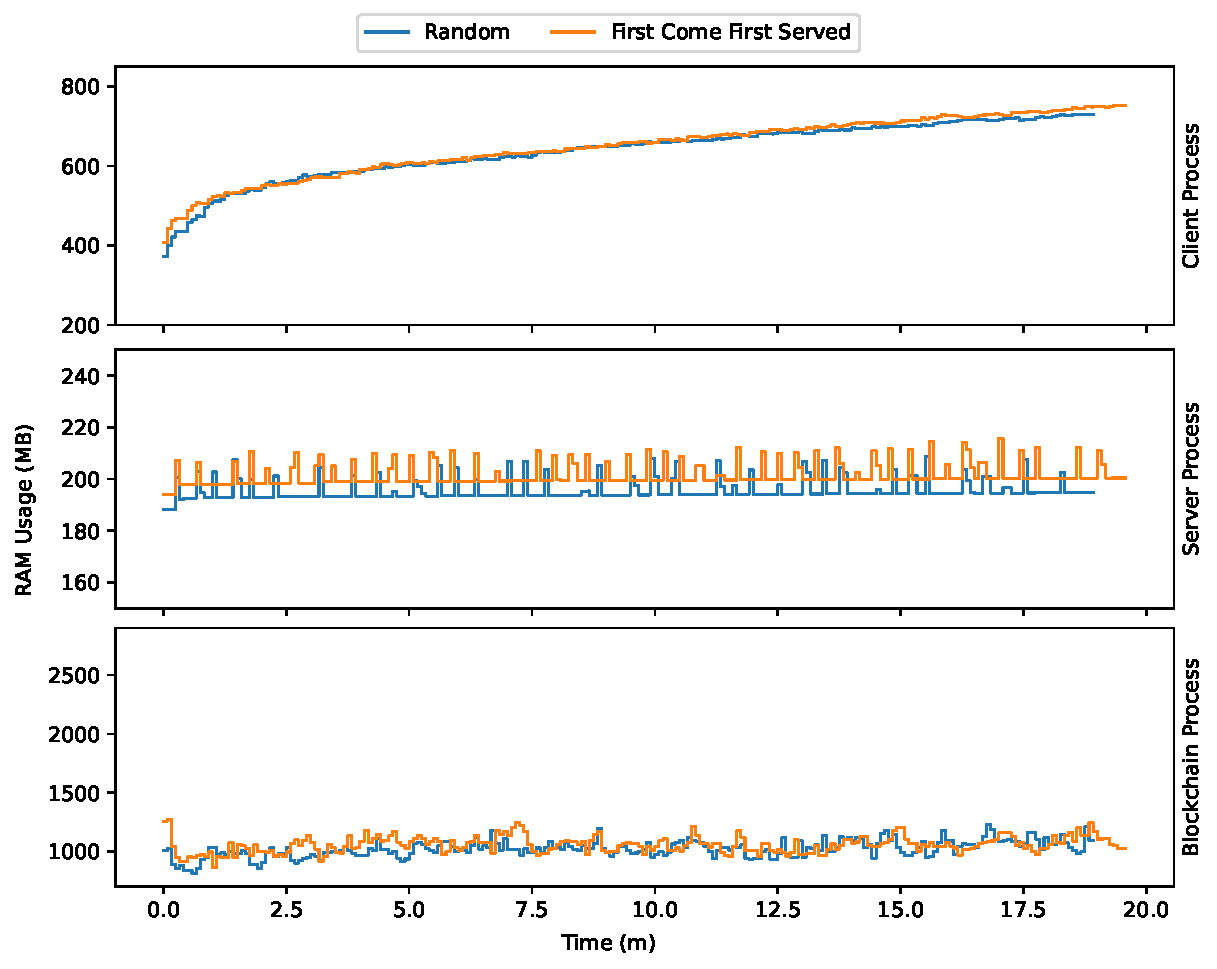
\includegraphics[width=0.8\textwidth]{graphics/selection/ram.pdf}
    \caption{RAM Usage Per Participant Selection Technique}
    \label{fig:ram_selection}
\end{figure}

\begin{figure}[!hpb]
    \centering
    \centering
    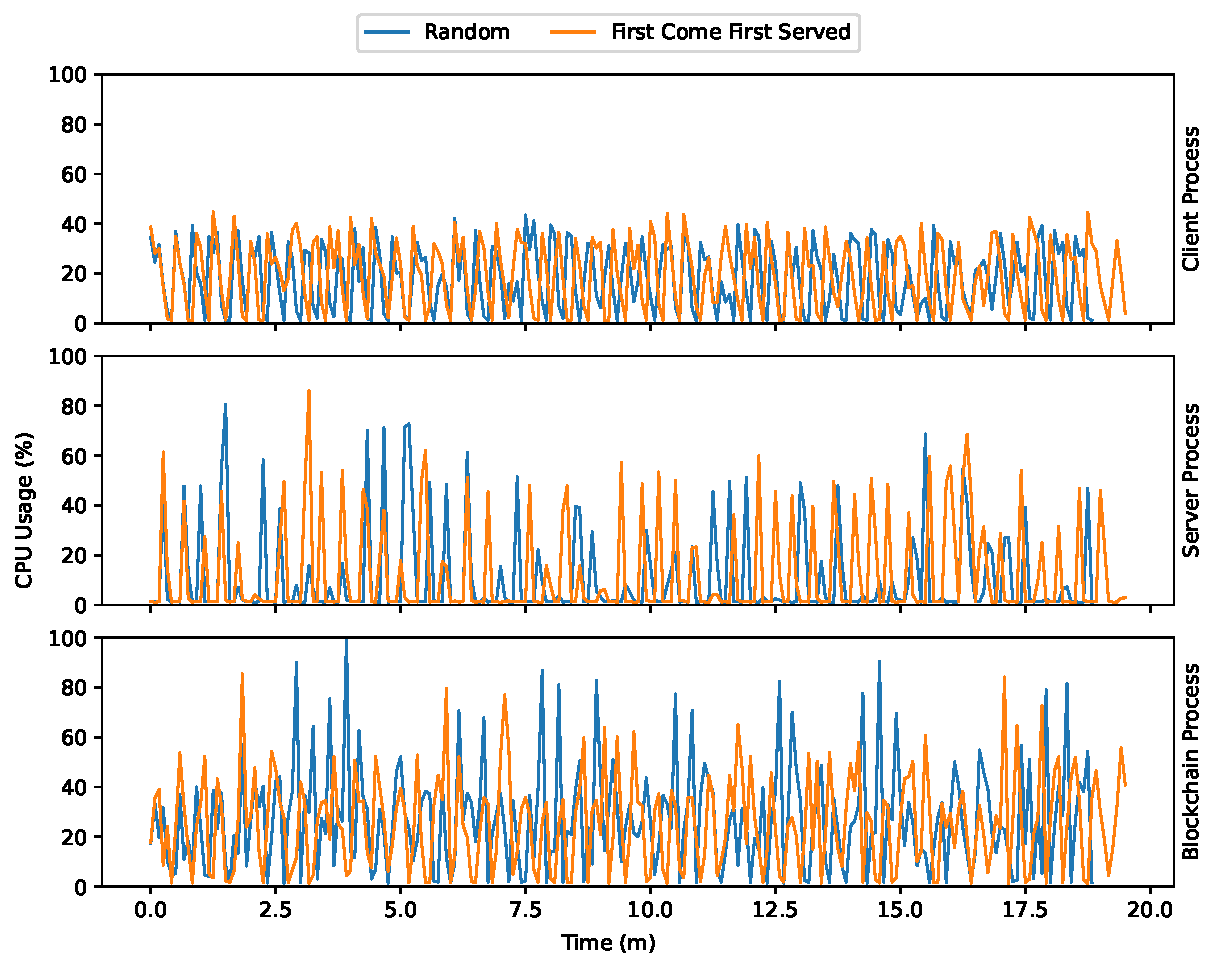
\includegraphics[width=0.8\textwidth]{graphics/selection/cpu.pdf}
    \caption{CPU Usage Per Participant Selection Technique}
    \label{fig:cpu_selection}
\end{figure}

\section{Conclusions and Improvements}

From this analysis, we can conclude that random selection performs better, in the sense that it allows for a more uniform selection of clients. This is crucial in \textit{non-iid} systems as each client has unique data. In addition, the "first come, first served" technique can also create a vector for vulnerability where more computationally powerful machines may be able to join more rounds if they end the training process earlier.

With that being said, a possible future improvement is to change the moment in which a devices registers for a "first come, first served" round: instead of joining after training, it would join before the round. This could, however, lead to another potential problem when devices in constrained networks would not be able to participate as the round would close the registrations before they were able to join it.

Finally, we can conclude that random selection seems to be the most fair as it allows for different devices to be selected equally if the randomness is provided by a uniform distribution.